\documentclass{article}
\usepackage[ngerman]{babel}
\usepackage{amsmath}
\usepackage{graphicx}
\usepackage{float}
\usepackage{xcolor}
\usepackage{mhchem}
\title{Physik Skript}
\author{}
\date{\today}

\begin{document}

\maketitle
\tableofcontents
\newpage



\section{Elektrostatik}
Ladungen sind immer an Teilchen mit einer Masse gebunden. Ein Ladungstransport stellt einen elektrischen Strom dar und Ladungstransport
ist immer mit Massentransport verbunden.
\begin{itemize}
\item negative Ladungen: Elektronen, negative Ionen 
\item positive Ladungen: Protonen, positive Ionen
\end{itemize}
Gleichartige Ladungen stoßen sich ab, entgegengesetzte Ladungen ziehen sich an. Alle Kräfte zwischen Atomen und Molekülen,
Festkörpern haben ihren Ursprung in Ladungen.\\

Die elektrische Ladung $q$ hat die Einheit Coulomb (SI-Einheit):
\begin{align}
    [q]=1\,\mathrm{C}=1\,\mathrm{A\,s}
\end{align}
Die Elementarladung $e$ hat den Wert:
\begin{align}
    e=1,6021892(46)\times 10^{-19}\,\mathrm{C}
\end{align}
Das Verhältnis der Elementarladung zur Masse eines Elektrons beträgt:
\begin{align}
    \frac{e}{m_\mathrm{e}}=1,7588047(49)\times 10^{11}\,\frac{\mathrm{C}}{\mathrm{Kg}}
\end{align}
Daraus folgt, dass die Masse eines Elektrons deutlich kleiner ist als der Wert der Elementarladung.
Die Ladung der Quarks ist ein Vielfaches der Ladung eines Protons/Elektrons und somit der Elementarladung.
\begin{align}
    q_\mathrm{up\, Quarks}&=\frac{2}{3}q_\mathrm{Proton}=\frac{2}{3}e\\
    q_\mathrm{down\, Quarks}&=\frac{1}{3}q_\mathrm{Elektron}=-\frac{1}{3}e
\end{align}
Die Ladung eines Protons ist gleich der Elementarladung und die Ladung eines Elektrons gleich der negativen Elementarladung.
\begin{align}
    q_\mathrm{Proton}=-q_\mathrm{Elektron}
\end{align}

\subsection{Ladungserhaltung}
In einem abgeschlossenen System bleibt die Gesamtladung zeitlich konstant, das heißt Ladungen können
werder erzeugt noch vernichtet werden. Es gilt der Satz von der Erhaltung der Gesamtladung:
\begin{align}
    \sum_{i=1}^N q_i=const.
\end{align}
Beispiele für die Ladungserhaltung ist der Neutronenzerfall.
Hier zerfällt ein Neutron mit der Ladung $q_\mathrm{n}=0$ in ein Proton
mit der Ladung $q_\mathrm{p}=+e$ und einem Elektron $q_e=-e$ und in ein Elektron-Antineutrino $q_{\,\overline{\nu}_e}=0$.
\begin{align}
    \ce{n -> p + e^- + \,\overline{\nu}_e}
\end{align}
Die Gesamtladung vor dem Zerfall betrug die des Neutrons, also gleich null. Nach dem Zerfall liegt die Ladung des Protons,
des Elektrons und des Elektron-Antineutrinos vor. 
\begin{align}
    q_\mathrm{nach}=e+(-e)+0=0
\end{align}
Somit ist die Gesamtladung vor dem Zerfall identisch mit der Ladung nach dem Zerfall.


\subsection{Coulomb Kraft}
Zwischen Ladungen wirken Kräfte, die von der Größe der Ladung und ihrem Abstand abhängen.
Die Elektrische Kraft zwischen zwei geladenen Teilchen wird durch das Coulomb Gesetz beschrieben:
\begin{align}
    \vec{F}=k\frac{q_1q_2}{r^2}\hat{r}
\end{align}
Die Kraft kann anziehend oder Abstoßend sein, je nach Art der Ladung.
Wenn 
\begin{itemize}
    \item $q_1\cdot q_2 < 0$ dann ist die Kraft anziehend
    \item $q_1\cdot q_2 > 0$ dann ist die Kraft abstoßend
\end{itemize}
$k$ ist definiert als 
\begin{align}
    k=\frac{1}{4\pi\varepsilon_0}=8,988\times 10^9\,\frac{\mathrm{Nm^2}}{\mathrm{C}^2}
\end{align}
$\epsilon_0$ beschreibt die Dielektrizitätskonstante des Vakuums mit 
\begin{align}
    \varepsilon_0=5,854188\times 10^{-12}\,\frac{\mathrm{C}}{\mathrm{V\,m}}
\end{align}
Innerhalb von Materie muss die Dielektrizitätskonstante $\epsilon$ des Mediums berücksichtigt werden.
Somit wird $k$ zu:
\begin{align}
    k=\frac{1}{4\pi\varepsilon(\omega)\varepsilon_0}
\end{align}
Für Wasser gilt zum Beispiel: $\varepsilon(0)=81$\\

\noindent Die Coulomb-Kraft ist eine Wechselwirkung. 
Die Quantenelektrodynamik beschreibt sie folgendermaßen:
\begin{center}
    ''\textit{Die elektromagnetische Wechselwirkung zwischen geladenen Teilchen (z.B. Elektronen)
    findet durch den Austausch von virtuellen Photonen statt.}''
\end{center}
Virtuelle Photonen sind keine ''klassischen Lichtteilchen'', sie existieren nur kurzzeitig während einer Wechselwirkung,
und können weder beobachtet noch nachgewiesen werden - sie sind ein mathematisches Modell, das die Wechselwirkung beschreibt.\\

\noindent Die Gravitaionskraft hat dieselbe Form wie das Coulombsche Gesetz. Die Gravitationskraft ist jedoch immer anziehend.
Sie wird beschrieben über: 
\begin{align}
    \vec{F}_{m_1\rightarrow m_2}=\gamma\frac{m_1m_2}{r^2}\hat{r}
\end{align}

Mit der Graviationskonstante $\gamma=6.67430(15)\times 10^{-11}\,\frac{\mathrm{m}^3}{\mathrm{Kg\,s^2}}$.
Für ein Elektron mit der Ladung $-e$, welches sich um ein Proton mit der Ladung $e$ bewegt gilt:
\begin{align}
    \frac{F_\mathrm{C}}{F_\mathrm{G}}
\end{align}
Also ist die Coulomb Kraft viel größer als die Gravitationskraft ($F_\mathrm{C}\gg F_\mathrm{G}$).

\subsection{Das Elektrische Feld}
Das Elektrische Feld $\vec{E}(\vec{r})$ ist durch die Kraft auf eine Probeladung $q$ definiert.
\begin{align}
    \vec{F}(\vec{r})=q\vec{E}(\vec{r})
\end{align}
Über die Coulomb Kraft ergibt sich für das Elektrische Feld einer Punktladung $Q$
\begin{align}
    \vec{F}(\vec{r})=k\frac{Q}{r^2}\hat{r}
\end{align}
Für positive Ladungen zeigt der Feldvektor nach außen, für negative Ladungen nach innen.
\begin{figure}[H]
    \centering
    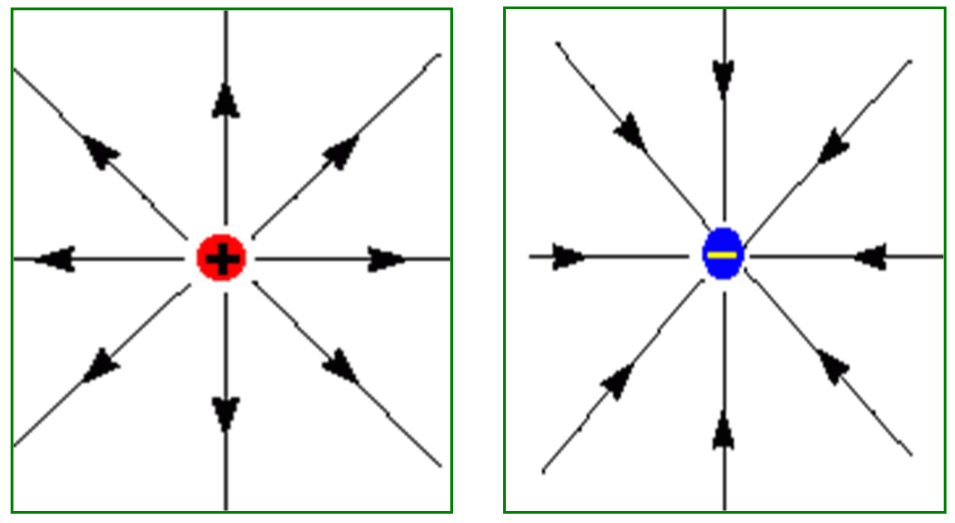
\includegraphics[width=0.80\textwidth]{Elektrisches Feld .png}
    \caption{Links nach außen gerichteter Feldvektor, rechts nach innen gerichteter Feldvektor.}
\end{figure}
Elektrische Feldlinien starten an positiven und enden an negativen Ladungen. 
Bei gleichen Ladungen stoßen sich die Feldlinien ab, bei entgegengesetzten Ladungen enden sie in der negativen Ladung.
Feldlinien können niemals bei der Ladung enden von der sie herkommen (keine geschlossenen Feldlinien).
\begin{figure}[H]
    \centering
    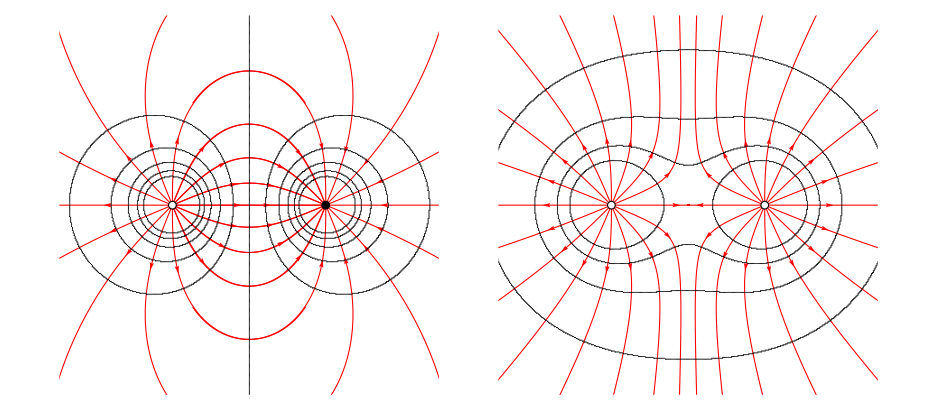
\includegraphics[width=0.80\textwidth]{Elektrisches Feld Ladungen.png}
    \caption{Links zwei entgegengesetzt Ladungen, Rechts zwei identische Ladungen}
\end{figure}

\subsection{Elektrische Leiter in einem elektrischen Feld}
Das Elektrische Feld im inneren eines geschlossenen Leiters ist immer null.
An der Oberfläche eines Leiters steht das elektrische Feld immer senkrecht zur Oberfläche.
Ein Beispiel für diese Eigenschaften ist der Faraday-Käfig.
\begin{figure}[H]
    \centering 
    \includegraphics[width=0.50\textwidth]{faraday käfig.png}
    \caption{Zu sehen ist, dass im inneren des Leiters das Elektrische Feld Null ist und die Feldlinien senkrecht zur Oberfläche stehen.}
\end{figure}

\subsection{Das Superpositionsprinzip}
Will man ein Elektrisches Feld für mehrere Ladungen berechen, so ergibt sich das resultierende Feld und Kraft 
durch die Überlagerung der einzel Felder.
Für das Elektrische Feld der Ladungen $q_i$ am Punkt $P$ (die Probeladung) gilt:
\begin{align}
    E_\mathrm{P}=k\cdot \sum_{i=1}^n \frac{q_i}{|\vec{r_i}|^2}\hat{r_i}
\end{align}
Die Kraft auf die Probeladung $q$ ergibt sich dann als:
\begin{align}
    \vec{F}=q\vec{E}_\mathrm{P}
\end{align}


\subsection{Spannung}
Die elektrische Spannung ist Arbeit im elektrischen Feld. Ihre Einheit ist $[\vec{E}]=\frac{\mathrm{V}}{\mathrm{m}}$.
Die Ladung q befindet sich in einem elektrischen Feld $\vec{E}(\vec{r})$ und soll von $\vec{r_1}$ nach $\vec{r_2}$ verschoben
werden. Dafür ist die Arbeit:
\begin{align}
    W&=\int_{\vec{r_1}}^{\vec{r_2}}\vec{F}(\vec{r})\,d\vec{r}\\
    &=q\int_{\vec{r_1}}^{\vec{r_2}}\vec{E}(\vec{r})\,d\vec{r}
\end{align}
notwendig.\\

\noindent Der Ausdruck des Integrals des Elektrischen Feldes wird als Potentialdifferenz ($U_2-U_1$) bezeichnet:
\begin{align}
    \int_{\vec{r_1}}^{\vec{r_2}}\vec{E}(\vec{r})\,d\vec{r}=U_2-U_1
\end{align}
Somit ergibt sich für die Arbeit $W$ im elektrostatischen Feld:
\begin{align}
    W&=q\int_{\vec{r_1}}^{\vec{r_2}}\vec{E}(\vec{r})\,d\vec{r}=q(U_2-U_1)
\end{align}
Die Arbeit in einem elektrostatischen Feld ist vom Weg unabhängig und hängt
nur vom Anfangspotential \( U_1 \) und Endpotential \( U_2 \) ab.
Ist dies gegeben, so handelt es sich um ein \textbf{konservatives Kraftfeld}.\\

\noindent In einem solchen Feld existiert ein Potential \( U(\vec{r}) \), aus dem das elektrische Feld berechnet werden kann:
\begin{align}
\vec{E}(\vec{r}) = -\vec{\nabla} U(\vec{r})
\end{align}

Diese Gleichung beschreibt, wie stark und in welche Richtung sich das Potential ändert.
Das \textbf{Minuszeichen} zeigt an, dass das elektrische Feld in Richtung des stärksten Abfalls des Potentials zeigt.\\

\noindent Das Potential einer Punktladung $Q$ lässt sich über 
\begin{align}
    U(\vec{r})=k\cdot\frac{Q}{r}\, \left(+U_0\right)
\end{align}
berechnen.\\

\noindent Die Spannung (Potentialdifferenz) ist nur definiert zwischen zwei Punkten.
Für die Potentialdifferenz zwischen Punkt $A$ und Punkt $B$ gilt:
\begin{align}
    U_{AB}=U(\vec{r_2})-U(\vec{r_1})=\frac{Q}{4\pi\varepsilon_0}\left(\frac{1}{r_2}-\frac{1}{r_1}\right)
\end{align}
Ist das Potential gleich Null, so liegt der Punkt im unendlichen. 
\begin{align}
    \lim_{r\to\infty}U(\vec{r})=0
\end{align}
Also: umso weiter weg man von einer Punktladung geht, desto kleiner wird das Potential.

\subsection{Plattenkondensator}
\begin{figure}[H]
    \centering
    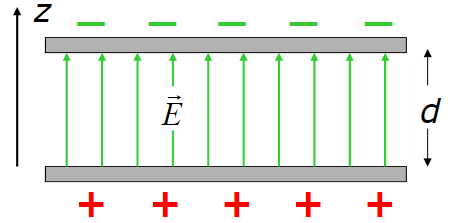
\includegraphics[width=0.6\textwidth]{Plattenkondensator.png}
    \caption{Der Aufbau eines Plattenkondensators mit der $z$-Achse}
\end{figure}
Bei einem Plattenkondensator gibt es zwei parallele, gegengesetzt geladene Metallplatten im Abstand $d$.
Diese bilden einen Kondensator aus.
Die Feldvektoren stehen senkrecht auf der positiv geladenen Platte und sind senkrecht auf die negative Platte gerichtet.
Sie entsprechen dem Einheitsvekor in $z$-Richtung:
\begin{align}
    \vec{E}\,||\,\hat{e}_z
\end{align}
Zudem ist das Elektrische Feld konstant, also homogen (überall gleich stark und gleiche Richtung) im inneren des Kondensators.
\begin{align}
    \vec{E}(\vec{r})=\vec{E}_0=const.\label{Plattenkondensator homogen}
\end{align}
Die Potenzialdifferenz (Spannung) zwischen den Platten ist:
\begin{align}
    \Delta U&=\int_0^d E(z)\,dz\\
    &=E_0\int_{0}^{d}dz\label{E_0 rausziehen}\\
    &=E_0\cdot d
\end{align}
Schritt~\ref{E_0 rausziehen} geht auf Grund des homogenen Feldes innerhalb des Plattenkondensators (siehe Formel~\ref{Plattenkondensator homogen}).
Für das Feld folgt damit:
\begin{align}
    E_0=\frac{\Delta U}{d}
\end{align}
Für die Einheit des elektrischen Feldes gilt $[E]=\frac{\mathrm{V}}{\mathrm{m}}$.
Bei Platten endlicher länge, ist das Feld am Rand (also Rechts und links) inhomogen.

\subsubsection{Beweis für die homogenität des elektrischen Feldes des Plattenkondensators}
Man betrachte eine Probeladung $q$ die sich im Abstand $a$ über einer großen Fläche mit 
gleichmäßiger Flächenladungsdichte $\sigma$ befindet.\\
Diese Fläche trägt eine Ladung:
\begin{align}
    dQ=\sigma\cdot da
\end{align}
Die Probeladung spürt eine Kraft durch das elektrische Feld dieser Fläche.
\begin{align}
    dF=k\cdot\frac{q\cdot dQ}{b^2}=k\cdot \frac{q\cdot \sigma\cdot dA}{b^2}
\end{align}
dabei ist $b$ der Abstand zwischen Probeladung und einem infinitesimal kleinen Flächenelement $dA$.\\

\noindent Nun zerlegt man die Kraft in zwei Richtungen. 
Einmal senkrecht zur Fläche (wirksame Kaft)
\begin{align}
    dF_s=dF\cdot \cos \alpha
\end{align}
und einmal Parallel zur Fläche (Symmetrische Kraft, diese hebt sich auf.)
\begin{align}
    dF_p=dF\cdot \sin \alpha=0
\end{align}
Die Symmetrische Kraft hebt sich auf, da alle horizontalen Anteile der Kräfte von gegenüberliegenden
Flächenelementen kompensiert werden.\\

\noindent Nun wird ein Ring mit Radius $r$ und Breite $dr$ betrachtet. Für die Fläche gilt:
\begin{align}
    dA=2\pi r\,dr
\end{align}
Es gelten folgende Beziehungen:
\begin{align}
    r=a\cdot\tan\alpha\\
    b=\frac{a}{\cos\alpha}
\end{align}
Die Ableitung von $r$ nach $\alpha$:
\begin{align}
    \frac{dr}{d\alpha}=\frac{a}{\cos^2\alpha}
\end{align}
Eingesetzt in $dF_s$ mit anschließendem Umformen und Integrieren gibt:
\begin{align}
    F=\frac{q\cdot \sigma}{2\varepsilon_0}
\end{align}
Somit haben wir bewiesen, dass die Kraft unabhängig von $a$ ist und somit konstant ist.
Somit ist das Feld eines idealen Plattenkondensators homogen.\\

\noindent Für die Kraft zweier Platten mit Ladung $Q$ gilt:
\begin{align}
    E=\frac{\sigma}{\varepsilon_0}=\frac{Q}{\varepsilon_0\cdot A}
\end{align}

\subsection{Kapazität}
Die Kapazität $C$ ist ein Maß dafür, wieviel Ladung man in einem Kondensator bei konstanter Spannung speichern kann.\\
Für das elektrische Feld gilt:
\begin{align}
    E&=\frac{U}{d}\\
    &=\frac{Q}{\varepsilon_0A}
\end{align}
Die Kapazität $C$ ist nun das Verhältnis zwischen der Ladung $Q$ und der Spannung $U$
\begin{align}
    C&=\frac{Q}{U}\\
    &=\frac{A\varepsilon_0}{d}
\end{align}
Diese Kapazität $C$ hängt nur von der Geometrie ab.
Ihre Einheit ist Farad $[C]=1\,\mathrm{F}=1\frac{\mathrm{A\,s}}{V}$
\begin{figure}[H]
    \centering
    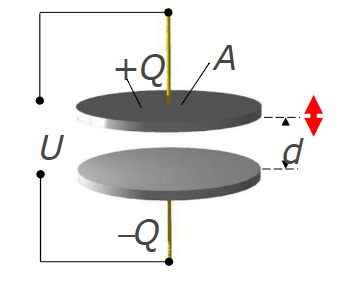
\includegraphics[width=0.40\textwidth]{aufbau plattenkondensator.png}
    \caption{Aufbau eines Plattenkondensators mit seinen relevanten Größen.}
\end{figure}

\subsection{Schaltzeichen eines Plattenkondensators}
\begin{figure}[H]
    \centering
    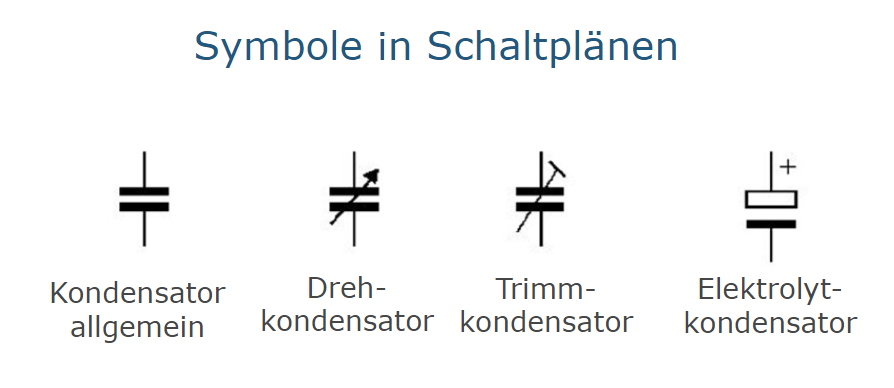
\includegraphics[width=0.8\textwidth]{Plattenkondensator schaltplan.png}
\end{figure}






\end{document}
